\section{INLA for Gaussian Data}
\todo[color = yellow]{Hvis du fokuserer på å få inn alle plottene og skrive innn likningene så kan jeg vet skrive forståelsestingene på tirsdag. I hvert fall er det fint om du tar det i den rekkefølgen :D  }
- It is a latent gausian model, these are a subclass of the structured additive regression models - > y belongs to the exponential family. In addition all latent variabler have gausian priors. 

%Dette er structured additiv model
\begin{equation}
\begin{split}
    g(\mu_i) = \eta_i = \alpha + \sum_{k = 1}^{n_\beta} \beta_k z_{mi} + \sum_{j = 1}^{n_f}f^{(j)}(u_{ji}) + \epsilon_i
\end{split}
\end{equation}

- i tillegg må the latent field være cond indep, i vårt tilfelle være $\eta_i$ ene
- siste punkt er få hyperparametere

\subsection{Plotting the data}
 
\begin{figure}[h]
    \centering
    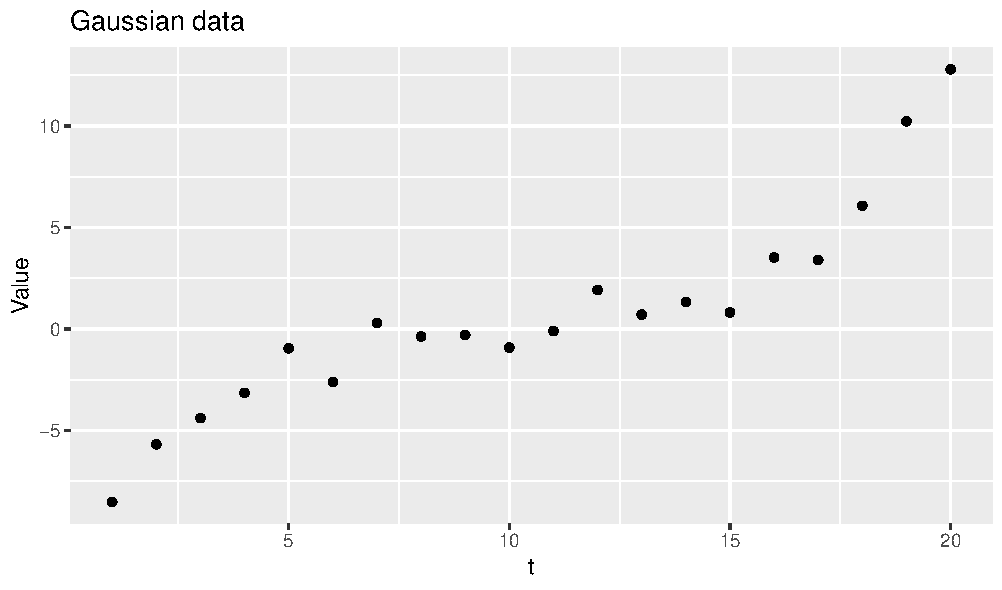
\includegraphics[width=\textwidth]{Images/gaussian_data.pdf}
    \caption{A simple plot of the data set "Gaussiandata.txt", given in the problem.}
    \label{fig:gaussian_data}
\end{figure}

- skriv in hva pressicion matrixen Q blir

%As $f|\theta$ is Gaussian distributed with mean $0$ and precision matrix $\textbf{Q}(\theta)$, we need to define the precision matrix of the model in order to use INLA. The precision matrix is defined as 



\subsection{Latent Gaussian model, and the possibility of using INLA to estimate the parameters in the model}




\subsection{Implementing a block Gibbs sampling algorithm for $f(\eta, \theta |y)$}

- skriv inn the full conditional for $\pi(\theta|\eta, y)$ og $\pi(\eta|\theta, y)$

%To implement block Gibbs sampling for $f(\eta, \theta | y)$, we firstly need to find the full conditionals for $\pi(\theta|\eta, y)$ and $\pi(\eta|\theta, y)$. 

we want to implement a block Gibbs sampling for $f(\eta, \theta | y)$, using two different block proposals. Firstly, we propose a new value for $\theta$ using the full conditional $\pi(\theta|\eta, y)$. The full conditional for $\theta$ is 

\begin{align}
    \pi(\theta| \eta, y) = \pi(y|\eta) \cdot \pi(\eta|\theta) \cdot \pi(\theta) \propto \pi(\eta|\theta) \cdot \pi(\theta) \nonumber \\
    = \theta^{\frac{(T-2)}{2}} \cdot exp \Big( \eta^T Q \frac{\theta}{2} \eta \Big) \cdot exp(\theta) \nonumber \\
    = exp \Big(  \theta \big(1 + \frac{\eta^T Q \eta}{2}  \big) \theta^{\frac{(T-2)}{2}}  \Big), 
\end{align}

which is gamma distributed with shape parameter $\alpha = T/2$ and scale parameter $\beta = 1/(\frac{1}{2}\cdot (1 + \eta^T Q \eta))$.

Then, for the second block proposal we propose a new value for the $\eta$-vector. We again use the full conditional, this time for $\eta$. This is then 

\begin{align}
    \pi(\eta | \theta, y) = 
\end{align}

\subsubsection{Estimate for the posterior marginal for the hyperparameter $\pi(\theta|y)$}
\begin{figure}[h!]
    \centering
    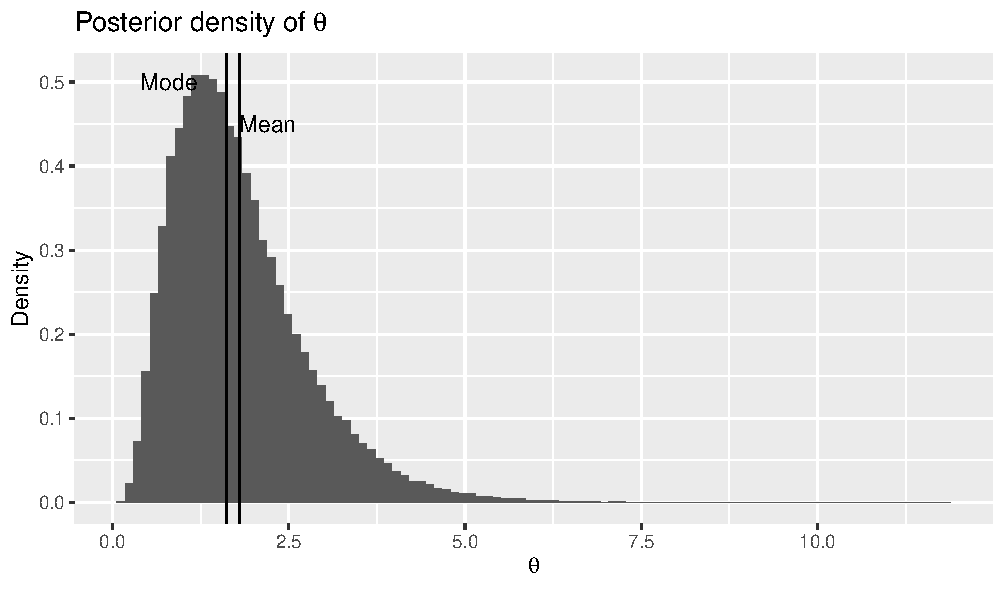
\includegraphics[width=\textwidth]{Images/post_theta_mcmc.pdf}
    \caption{Plot of the estimate for the posterior marginal for the hyperparameter $\pi(\theta|y)$.}
    \label{fig:post_theta_mcmc}
\end{figure}

\subsubsection{Estimate of the smooth effect using the mean and pointwise a $95 \%$ confidence bound around the mean}
\begin{figure}[h]
    \centering
    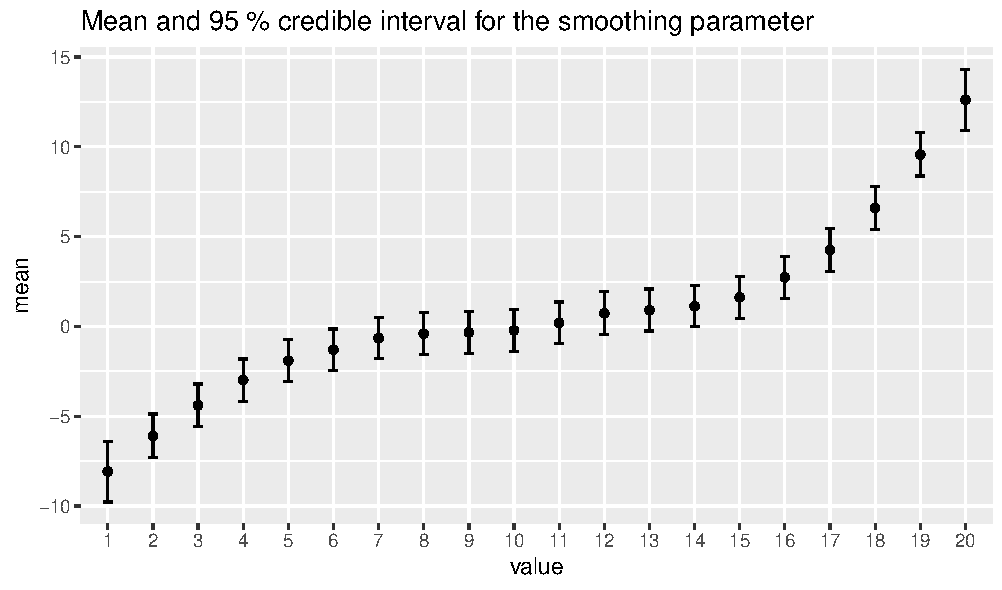
\includegraphics[width=\textwidth]{Images/post_eta_mcmc.pdf}
    \caption{Plot of the mean and the $95\%$ credible interval for the smoothing parameter $\eta$. }
    \label{fig:post_eta_mcmc}
\end{figure}

\subsection{Approximating the posterior marginal for the hyperparameter $\theta$, $\pi(\theta|y)$ using the INLA scheme}

\begin{figure}[h!]
    \centering
    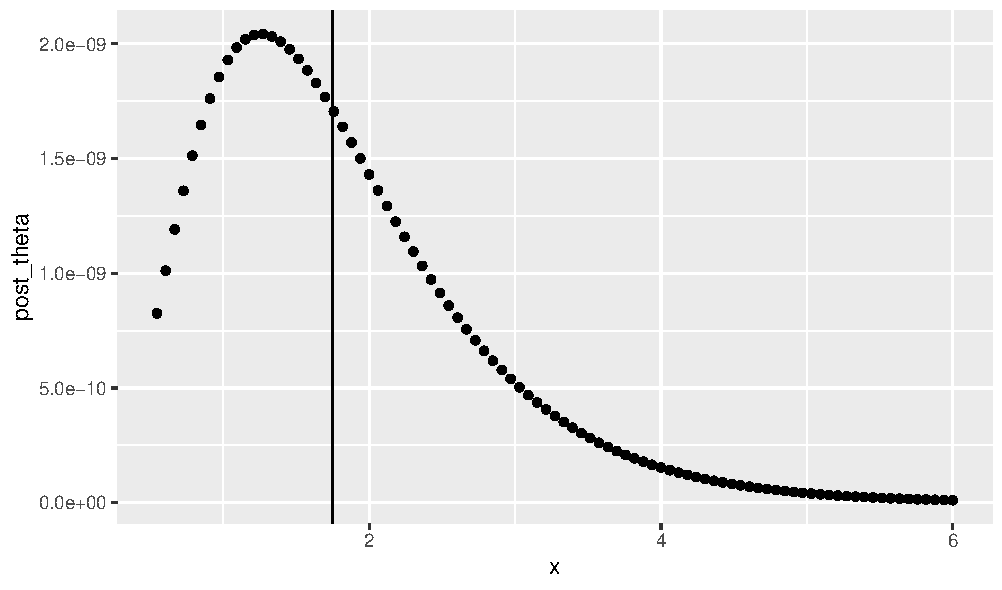
\includegraphics[width=\textwidth]{Images/post_theta_inla.pdf}
    \caption{Plot of the estimate for the posterior marginal for the hyperparameter $\pi(\theta|y)$ using the INLA scheme.}
    \label{fig:post_theta_inla}
\end{figure}
 
 
\subsubsection{Approximation for $\pi(\theta|y)$}


- veldig mye av disse tingene står som kladd i de pdf ene jeg sendte deg så se gjerne der for inspirasjon-


\subsection{Implementing the approximation of the marginal posterior for the smooth effect, $\pi(\eta_i | y)$}

\begin{figure}[h!]
    \centering
    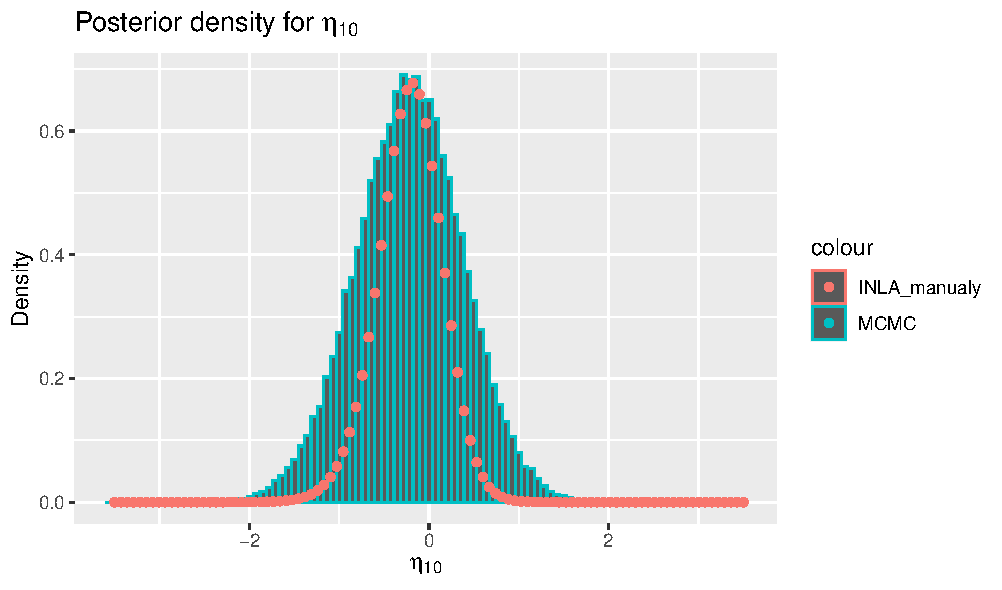
\includegraphics[width=\textwidth]{Images/post_eta_inla.pdf}
    \caption{Plot of the estimate for the posterior marginal for the smoothing effect $\pi(\eta_i|y)$ using the INLA scheme.}
    \label{fig:post_eta_inla}
\end{figure}



\subsection{Using the inla() - function in R to implement the model,and comparing the results}


\begin{figure}[h]
    \centering
    \includegraphics{}
    \caption{Caption}
    \label{fig:my_label}
\end{figure}

\begin{figure}[h]
    \centering
    \includegraphics{}
    \caption{Caption}
    \label{fig:my_label}
\end{figure}

\begin{figure}[h]
    \centering
    \includegraphics{}
    \caption{Caption}
    \label{fig:my_label}
\end{figure}

\begin{figure}[h]
    \centering
    \includegraphics{}
    \caption{Caption}
    \label{fig:my_label}
\end{figure}
